% answers.tex —— 1977 年·江苏无锡市初试卷 · 参考答案与详细解析片段
% 由 tools/generate_projects.py 依来源总账自 1977/1977_数学真题_江苏无锡市初试_试题.md + 1977/1977_数学真题_江苏无锡市初试_解析正文.md + 1977/1977_数学真题_江苏无锡市初试_答案要点.md 生成，勿手改（改源 MD 后重跑）


\begin{gktip}
固定源为试题汇编扫描件，仅含题面、无解答，下文逐题独立推导。原卷第三大题第 3 小问印作「当 $x$ 为何值时」，字面保留、依题意按 $m$ 求解（见试题源注）；第八题结论 $AC^2=AO\cdot AD$ 经复核为原卷字面即成立（推导见第 8 题），不作更正。
\end{gktip}

\begin{answer}
\gksolhead{1}{}

\textbf{题目}（18 分）：

回答下列问题：

（1） 求代数式 $f(x)=3x^2-2x-5$ 的值，当 $x=0$ 时，$f(0)=\underline{\hspace{2.5em}}$；当 $x=-1$ 时，$f(-1)=\underline{\hspace{2.5em}}$；当 $x=\dfrac13$ 时，$f\left(\dfrac13\right)=\underline{\hspace{2.5em}}$。

（2） 在 $\mathrm{Rt}\triangle ABC$ 中，已知 $\angle C=90^\circ$，$AB=13$，$BC=5$，则 $\sin A=\underline{\hspace{2em}}$，$\cos B=\underline{\hspace{2em}}$；$\operatorname{tg}A=\underline{\hspace{2em}}$，$\operatorname{ctg}A=\underline{\hspace{2em}}$。

（3） 化简：$\sqrt{(3-x)^2}$；

（4） 已知圆方程为 $x^2+y^2=25$，那么这个圆以原点为极点，$x$ 轴的正方向为极轴的极坐标方程是 $\underline{\hspace{3em}}$，圆心的极坐标是 $\underline{\hspace{2em}}$。

（5） 已知长方体的长、宽、高分别是 $3\,\mathrm{cm}$、$2\,\mathrm{cm}$、$5\,\mathrm{cm}$，则它的体积为 $\underline{\hspace{2.5em}}$，它的表面积为 $\underline{\hspace{2.5em}}$。

\Needspace{4\baselineskip}
\textbf{解析}

\gksubpart{（1）}

\Needspace{5\baselineskip}
逐个代入 $f(x)=3x^2-2x-5$：

\nopagebreak[4]
\[
f(0)=3\cdot 0^2-2\cdot 0-5=-5,
\]

\nopagebreak[4]
\[
f(-1)=3\cdot(-1)^2-2\cdot(-1)-5=3+2-5=0,
\]

\nopagebreak[4]
\[
f\left(\frac13\right)=3\cdot\frac19-2\cdot\frac13-5=\frac13-\frac23-5=-\frac{16}{3}.
\]

\gksubpart{（2）}

\Needspace{5\baselineskip}
$\angle C=90^\circ$，$AB=13$ 为斜边，$BC=5$，由勾股定理

\nopagebreak[4]
\[
AC=\sqrt{13^2-5^2}=\sqrt{144}=12.
\]

\Needspace{5\baselineskip}
于是

\nopagebreak[4]
\[
\sin A=\frac{BC}{AB}=\frac5{13},\qquad
\cos B=\frac{BC}{AB}=\frac5{13},
\]

\nopagebreak[4]
\[
\operatorname{tg}A=\frac{BC}{AC}=\frac5{12},\qquad
\operatorname{ctg}A=\frac{AC}{BC}=\frac{12}{5}.
\]

\gksubpart{（3）}

\Needspace{5\baselineskip}
二次根式开方取绝对值：

\nopagebreak[4]
\[
\sqrt{(3-x)^2}=\left|3-x\right|
=\begin{cases}
3-x, & x\le 3,\\
x-3, & x>3.
\end{cases}
\]

\gksubpart{（4）}

\Needspace{5\baselineskip}
以原点为极点、$x$ 轴正方向为极轴时，$\rho^2=x^2+y^2$。代入 $x^2+y^2=25$ 得

\nopagebreak[4]
\[
\rho^2=25,
\qquad
\rho=5\quad(\rho\ge 0).
\]

圆心即原点，也就是极点，其极坐标为 $(0,0)$（$\rho=0$，极角 $\theta$ 任意）。

\gksubpart{（5）}

\nopagebreak[4]
\[
V=3\times 2\times 5=30\ (\mathrm{cm^3}),
\]

\nopagebreak[4]
\[
S=2\times(3\times 2+3\times 5+2\times 5)=2\times 31=62\ (\mathrm{cm^2}).
\]

\gkanswer{答案（1）：$f(0)=-5$；$f(-1)=0$；$f\left(\dfrac13\right)=-\dfrac{16}{3}$。}

\gkanswer{答案（2）：$\sin A=\dfrac5{13}$；$\cos B=\dfrac5{13}$；$\operatorname{tg}A=\dfrac5{12}$；$\operatorname{ctg}A=\dfrac{12}{5}$。}

\gkanswer{答案（3）：$\sqrt{(3-x)^2}=\left|3-x\right|$（$x\le 3$ 时为 $3-x$，$x>3$ 时为 $x-3$）。}

\gkanswer{答案（4）：极坐标方程 $\rho=5$；圆心的极坐标为 $(0,0)$（圆心即极点，极角任意）。}

\gkanswer{答案（5）：体积 $30\ \mathrm{cm^3}$；表面积 $62\ \mathrm{cm^2}$。}

\end{answer}
\begin{answer}
\gksolhead{2}{}

\textbf{题目}（16 分）：

计算：

（1） $\left[\left|8-6\right|-\left|4-7\right|\right]\times\dfrac{1}{\left|1-2\right|}$；

（2） $a^{\frac12}b^0\left(ab^2\right)^{-\frac12}\div\left[b^{\frac13}\left(a^3b^{-2}\right)^{-\frac13}\right]$；

（3） $\left(\lg 50\right)^2+\lg 2\lg 50^2+\left(\lg 2\right)^2$；

（4） $\sin 105^\circ+\sin 15^\circ$；

（5） $\lim\limits_{n\to\infty}\dfrac{5-2n+3n^2}{4n^2-n-7}$；

（6） $\sqrt{\dfrac{1-\cos\theta}{1+\cos\theta}}+\sqrt{\dfrac{1+\cos\theta}{1-\cos\theta}}$

\Needspace{4\baselineskip}
\textbf{解析}

\gksubpart{（1）}

\nopagebreak[4]
\[
\left[\left|8-6\right|-\left|4-7\right|\right]\times\frac{1}{\left|1-2\right|}
=(2-3)\times 1=-1.
\]

\gksubpart{（2）}

\Needspace{5\baselineskip}
分别化简被除式与除式：

\nopagebreak[4]
\[
a^{\frac12}b^0\left(ab^2\right)^{-\frac12}
=a^{\frac12}\cdot a^{-\frac12}\cdot b^{-1}=b^{-1},
\]

\nopagebreak[4]
\[
b^{\frac13}\left(a^3b^{-2}\right)^{-\frac13}
=b^{\frac13}\cdot a^{-1}\cdot b^{\frac23}=a^{-1}b.
\]

\Needspace{5\baselineskip}
故原式

\nopagebreak[4]
\[
b^{-1}\div\left(a^{-1}b\right)=b^{-1}\cdot a b^{-1}=\frac{a}{b^2}.
\]

\gksubpart{（3）}

\Needspace{5\baselineskip}
由 $\lg 50^2=2\lg 50$，原式为完全平方：

\nopagebreak[4]
\[
\left(\lg 50\right)^2+2\lg 2\lg 50+\left(\lg 2\right)^2
=\left(\lg 50+\lg 2\right)^2
=\left(\lg 100\right)^2=2^2=4.
\]

\gksubpart{（4）}

\Needspace{5\baselineskip}
和差化积：

\nopagebreak[4]
\[
\sin 105^\circ+\sin 15^\circ
=2\sin 60^\circ\cos 45^\circ
=2\cdot\frac{\sqrt3}{2}\cdot\frac{\sqrt2}{2}
=\frac{\sqrt6}{2}.
\]

\gksubpart{（5）}

\Needspace{5\baselineskip}
分子、分母同除以 $n^2$：

\nopagebreak[4]
\[
\lim_{n\to\infty}\frac{5-2n+3n^2}{4n^2-n-7}
=\lim_{n\to\infty}\frac{\dfrac5{n^2}-\dfrac2n+3}{4-\dfrac1n-\dfrac7{n^2}}
=\frac34.
\]

\gksubpart{（6）}

\Needspace{5\baselineskip}
分子有理化：

\nopagebreak[4]
\[
\sqrt{\frac{1-\cos\theta}{1+\cos\theta}}
=\frac{1-\cos\theta}{\sqrt{1-\cos^2\theta}},
\qquad
\sqrt{\frac{1+\cos\theta}{1-\cos\theta}}
=\frac{1+\cos\theta}{\sqrt{1-\cos^2\theta}},
\]

\Needspace{5\baselineskip}
相加得

\nopagebreak[4]
\[
\frac{2}{\sqrt{1-\cos^2\theta}}=\frac{2}{\left|\sin\theta\right|},
\]

在 $0<\theta<\pi$ 时即为 $\dfrac{2}{\sin\theta}$。

\gkanswer{答案（1）：$-1$。}

\gkanswer{答案（2）：$\dfrac{a}{b^2}$。}

\gkanswer{答案（3）：$4$。}

\gkanswer{答案（4）：$\dfrac{\sqrt6}{2}$。}

\gkanswer{答案（5）：$\dfrac34$。}

\gkanswer{答案（6）：$\dfrac{2}{\left|\sin\theta\right|}$}

\end{answer}
\begin{answer}
\gksolhead{3}{}

\textbf{题目}（11 分）：

解方程、方程组：

（1） $\dfrac{5}{x-2}+\dfrac{2}{x^2+2x}=\dfrac{20}{x^2-4}$；

（2） $\begin{cases} x-\dfrac{y-1}{2}=3 \\ \dfrac{x}{4}+y=4 \end{cases}$；

（3） 当 $x$ 为何值时，二次方程 $mx^2+3mx+3=0$：（1）有两个相等的实数根；（2）无实数根。

\begin{gktip}
\textbf{源注}：原卷印作「当 $x$ 为何值时」。该方程以 $x$ 为未知数、$m$ 为参数，依题意应为「当 $m$ 为何值时」。本文按原卷字面保留题干，解析按 $m$ 求解。
\end{gktip}

\Needspace{4\baselineskip}
\textbf{解析}

\gksubpart{（1）}

\Needspace{5\baselineskip}
两边同乘以最简公分母 $x(x-2)(x+2)$：

\nopagebreak[4]
\[
5x(x+2)+2(x-2)=20x,
\]

\nopagebreak[4]
\[
5x^2+10x+2x-4-20x=0
\quad\Longrightarrow\quad
5x^2-8x-4=0
\quad\Longrightarrow\quad
(5x+2)(x-2)=0.
\]

得 $x=-\dfrac25$ 或 $x=2$；$x=2$ 使分母 $x-2$ 为零，是增根，舍去，故 $x=-\dfrac25$。

\gksubpart{（2）}

\Needspace{5\baselineskip}
由第二个方程得 $x=16-4y$，代入第一个方程：

\nopagebreak[4]
\[
16-4y-\frac{y-1}{2}=3
\quad\Longrightarrow\quad
32-8y-y+1=6
\quad\Longrightarrow\quad
9y=27,
\]

故 $y=3$，从而 $x=16-4\times 3=4$。

\gksubpart{（3）}

\Needspace{5\baselineskip}
按题意求参数 $m$（原卷字面印作「当 $x$ 为何值时」，见试题源注）。方程 $mx^2+3mx+3=0$ 是关于 $x$ 的二次方程，需 $m\ne 0$，其判别式

\nopagebreak[4]
\[
\Delta=(3m)^2-4\cdot m\cdot 3=9m^2-12m=3m(3m-4).
\]

（1）有两个相等的实数根，需 $\Delta=0$：$m=\dfrac43$（$m=0$ 时方程退化为 $3=0$，无根，不合）。

\Needspace{5\baselineskip}
（2）无实数根，需 $\Delta<0$：即 $3m(3m-4)<0$，得

\nopagebreak[4]
\[
0<m<\frac43.
\]

\gkanswer{答案（1）：$x=-\dfrac25$。}

\gkanswer{答案（2）：$x=4$，$y=3$。}

\gkanswer{答案（3）：有两个相等的实数根时 $m=\dfrac43$；无实数根时 $0<m<\dfrac43$。}

\end{answer}
\begin{answer}
\gksolhead{4}{}

\textbf{题目}（8 分）：

分别写出数列 $1$，$3$，$5$，$7$，$\cdots\cdots$ 和 $1$，$\dfrac12$，$\dfrac14$，$\dfrac18$，$\cdots\cdots$ 的通项公式，并用求和公式计算：$1+1$，$3+\dfrac12$，$5+\dfrac14$，$7+\dfrac18$，$\cdots\cdots$，前 $10$ 项的和。

\Needspace{4\baselineskip}
\textbf{解析}

\Needspace{5\baselineskip}
第一个数列是首项 $1$、公差 $2$ 的等差数列，通项

\nopagebreak[4]
\[
a_n=1+(n-1)\cdot 2=2n-1;
\]

\Needspace{5\baselineskip}
第二个数列是首项 $1$、公比 $\dfrac12$ 的等比数列，通项

\nopagebreak[4]
\[
b_n=\left(\frac12\right)^{n-1}=\frac{1}{2^{n-1}}.
\]

\Needspace{5\baselineskip}
和式中第 $k$ 项为 $\left(2k-1\right)+\dfrac{1}{2^{k-1}}$，前 $10$ 项和用两个求和公式分别计算：

\nopagebreak[4]
\[
\sum_{k=1}^{10}(2k-1)=\frac{10\times(1+19)}{2}=100,
\]

\nopagebreak[4]
\[
\sum_{k=1}^{10}\frac{1}{2^{k-1}}
=\frac{1-\left(\frac12\right)^{10}}{1-\frac12}
=2-\frac{1}{512}
=\frac{1023}{512}.
\]

\Needspace{5\baselineskip}
故

\nopagebreak[4]
\[
S_{10}=100+\frac{1023}{512}=\frac{52223}{512}\approx 102.
\]

\gkanswer{答案：两数列通项分别为 $a_n=2n-1$ 与 $b_n=\dfrac{1}{2^{n-1}}$；前 $10$ 项之和 $S_{10}=\dfrac{52223}{512}\approx 102$。}

\end{answer}
\begin{answer}
\gksolhead{5}{}

\textbf{题目}（8 分）：

在 $\triangle ABC$ 中，$\angle A=60^\circ$，$AB=2$，$AC=1+\sqrt3$，解这个三角形。

\Needspace{4\baselineskip}
\textbf{解析}

\Needspace{5\baselineskip}
记 $a=BC$，$b=CA=1+\sqrt3$，$c=AB=2$。由余弦定理，

\nopagebreak[4]
\[
a^2=b^2+c^2-2bc\cos A
=(1+\sqrt3)^2+4-2(1+\sqrt3)\times 2\times\frac12
=4+2\sqrt3+4-2-2\sqrt3=6,
\]

\Needspace{5\baselineskip}
故

\nopagebreak[4]
\[
a=\sqrt6.
\]

\Needspace{5\baselineskip}
由正弦定理求角 $B$：

\nopagebreak[4]
\[
\sin B=\frac{b\sin A}{a}
=\frac{(1+\sqrt3)\sin 60^\circ}{\sqrt6}
=\frac{\sqrt3+3}{2\sqrt6}
=\frac{\sqrt6+\sqrt2}{4}=\sin 75^\circ.
\]

\Needspace{5\baselineskip}
$\sin B$ 的值对应 $75^\circ$ 与 $105^\circ$ 两个可能角，用余弦定理判定：

\nopagebreak[4]
\[
\cos B=\frac{a^2+c^2-b^2}{2ac}
=\frac{6+4-(4+2\sqrt3)}{4\sqrt6}
=\frac{6-2\sqrt3}{4\sqrt6}>0,
\]

\Needspace{5\baselineskip}
故 $B$ 为锐角，$B=75^\circ$。于是

\nopagebreak[4]
\[
C=180^\circ-60^\circ-75^\circ=45^\circ.
\]

\gkanswer{答案：$a=\sqrt6$，$B=75^\circ$，$C=45^\circ$。}

\end{answer}
\begin{answer}
\gksolhead{6}{}

\textbf{题目}（8 分）：

把底面半径和高均为 $a$ 的一个圆柱体和圆锥体的金属物体，熔铸成一个金属球，求这个球的半径（损耗不计）。

\Needspace{4\baselineskip}
\textbf{解析}

\Needspace{5\baselineskip}
圆柱体底面半径 $a$、高 $a$，圆锥体底面半径 $a$、高 $a$，两者体积之和

\nopagebreak[4]
\[
V_{\text{\text{圆柱}}}+V_{\text{\text{圆锥}}}
=\pi a^2\cdot a+\frac13\pi a^2\cdot a
=\frac43\pi a^3.
\]

\Needspace{5\baselineskip}
熔铸成半径 $R$ 的金属球，体积不变：

\nopagebreak[4]
\[
\frac43\pi R^3=\frac43\pi a^3
\quad\Longrightarrow\quad
R^3=a^3,
\]

\Needspace{5\baselineskip}
故球的半径

\nopagebreak[4]
\[
R=a.
\]

\gkanswer{答案：$R=a$。}

\end{answer}
\begin{answer}
\gksolhead{7}{}

\textbf{题目}（11 分）：

\Needspace{5\baselineskip}
如果直线的倾角 $\alpha$ 满足 $4\sin\alpha=3\cos\alpha$，并过椭圆

\nopagebreak[4]
\[
\frac{x^2}{16}+\frac{y^2}{25}=1
\]

的焦点，求直线方程以及直线与坐标轴围成的三角形的面积。

\Needspace{4\baselineskip}
\textbf{解析}

\Needspace{5\baselineskip}
由 $4\sin\alpha=3\cos\alpha$ 得 $\tan\alpha=\dfrac34$；倾角 $\alpha\in[0,\pi)$，故 $\alpha$ 为锐角，

\nopagebreak[4]
\[
\sin\alpha=\frac35,\qquad \cos\alpha=\frac45,
\]

直线的斜率 $k=\tan\alpha=\dfrac34$。

\Needspace{5\baselineskip}
椭圆 $\dfrac{x^2}{16}+\dfrac{y^2}{25}=1$ 中 $a^2=25$、$b^2=16$，焦点在 $y$ 轴上，

\nopagebreak[4]
\[
c=\sqrt{25-16}=3,
\]

两焦点为 $(0,3)$、$(0,-3)$。

\Needspace{5\baselineskip}
过焦点 $(0,3)$、斜率 $\dfrac34$ 的直线为 $y=\dfrac34x+3$，即

\nopagebreak[4]
\[
3x-4y+12=0;
\]

过焦点 $(0,-3)$ 时为 $y=\dfrac34x-3$，即 $3x-4y-12=0$。

\Needspace{5\baselineskip}
以 $3x-4y+12=0$ 为例：它在 $x$ 轴、$y$ 轴上的截距分别为 $-4$ 和 $3$，与两坐标轴围成直角三角形，

\nopagebreak[4]
\[
S=\frac12\times 4\times 3=6;
\]

直线 $3x-4y-12=0$ 的截距为 $4$ 和 $-3$，面积同为 $6$。故所求直线方程为 $3x-4y+12=0$ 或 $3x-4y-12=0$，围成的三角形面积为 $6$。

\gkanswer{答案：直线方程为 $3x-4y+12=0$（过焦点 $(0,3)$）或 $3x-4y-12=0$（过焦点 $(0,-3)$）；直线与坐标轴围成的三角形面积为 $6$。}

\end{answer}
\begin{answer}
\gksolhead{8}{}

\textbf{题目}（8 分）：

\Needspace{5\baselineskip}
在 $\odot O$ 中，直径 $AB$ 和弦 $AC$ 的夹角为 $30^\circ$，切线 $CD$ 和 $AB$ 的延长线交于 $D$，求证：

\nopagebreak[4]
\[
AC^2=AO\cdot AD.
\]
\nopagebreak[4]
\begin{center}% 1977 年江苏无锡市初试卷第八题：圆 O、直径 AOB、弦 AC 与切线 CD，
% 切线与 AB 的延长线交于 D（按源卷第 3 页布局：C 在圆的右上方，D 在 B 右侧）
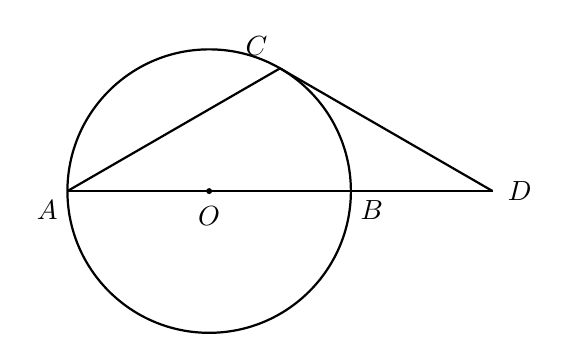
\begin{tikzpicture}[scale=0.9]
  % 半径 R=2，圆心 O=(2,0)；C 在圆心角 60° 处：C=(2+2cos60°, 2sin60°)=(3,1.732)
  % 切线 CD 与 x 轴交于 D=(6,0)
  \coordinate (A) at (0,0);
  \coordinate (O) at (2,0);
  \coordinate (B) at (4,0);
  \coordinate (C) at (3,1.732);
  \coordinate (D) at (6,0);
  \draw[thick] (O) circle (2);
  \draw[thick] (A) -- (D);
  \draw[thick] (A) -- (C);
  \draw[thick] (C) -- (D);
  \fill (O) circle (1.2pt) node[below=2pt] {$O$};
  \node[below left] at (A) {$A$};
  \node[below right] at (B) {$B$};
  \node[above left=1pt] at (C) {$C$};
  \node[right=2pt] at (D) {$D$};
\end{tikzpicture}
\end{center}
\nopagebreak[4]
\Needspace{4\baselineskip}
\textbf{解析}
\nopagebreak[4]
\begin{center}% 1977 年江苏无锡市初试卷第八题：圆 O、直径 AOB、弦 AC 与切线 CD，
% 切线与 AB 的延长线交于 D（按源卷第 3 页布局：C 在圆的右上方，D 在 B 右侧）
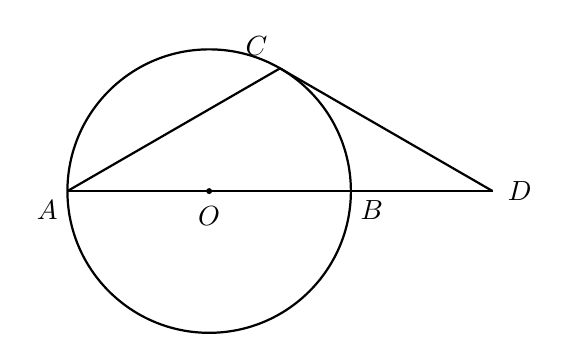
\begin{tikzpicture}[scale=0.9]
  % 半径 R=2，圆心 O=(2,0)；C 在圆心角 60° 处：C=(2+2cos60°, 2sin60°)=(3,1.732)
  % 切线 CD 与 x 轴交于 D=(6,0)
  \coordinate (A) at (0,0);
  \coordinate (O) at (2,0);
  \coordinate (B) at (4,0);
  \coordinate (C) at (3,1.732);
  \coordinate (D) at (6,0);
  \draw[thick] (O) circle (2);
  \draw[thick] (A) -- (D);
  \draw[thick] (A) -- (C);
  \draw[thick] (C) -- (D);
  \fill (O) circle (1.2pt) node[below=2pt] {$O$};
  \node[below left] at (A) {$A$};
  \node[below right] at (B) {$B$};
  \node[above left=1pt] at (C) {$C$};
  \node[right=2pt] at (D) {$D$};
\end{tikzpicture}
\end{center}
\nopagebreak[4]
\Needspace{5\baselineskip}
设圆 $O$ 的半径为 $R$，连接 $OC$。$CD$ 为过 $C$ 的切线，故

\nopagebreak[4]
\[
OC\perp CD.
\]

\Needspace{5\baselineskip}
圆周角 $\angle BAC=30^\circ$ 对弧 $BC$，所以圆心角

\nopagebreak[4]
\[
\angle BOC=2\times 30^\circ=60^\circ.
\]

\Needspace{5\baselineskip}
等腰三角形 $AOC$ 中（$OA=OC=R$），

\nopagebreak[4]
\[
\angle CAO=\angle ACO=30^\circ,
\]

\Needspace{5\baselineskip}
从而

\nopagebreak[4]
\[
\angle ACD=\angle ACO+\angle OCD=30^\circ+90^\circ=120^\circ.
\]

\Needspace{5\baselineskip}
在 $\triangle ACD$ 中，

\nopagebreak[4]
\[
\angle ADC=180^\circ-30^\circ-120^\circ=30^\circ.
\]

\Needspace{5\baselineskip}
于是 $\angle ACO=\angle ADC=30^\circ$，又 $\angle CAD$ 公共，得

\nopagebreak[4]
\[
\triangle ACO\sim\triangle ADC,
\]

\Needspace{5\baselineskip}
对应边成比例：

\nopagebreak[4]
\[
\frac{AO}{AC}=\frac{AC}{AD}
\quad\Longrightarrow\quad
AC^2=AO\cdot AD.
\]

这正是原卷要求证明的结论（复核：$AD=AO+OD$，而 $\mathrm{Rt}\triangle OCD$ 中 $\angle COD=60^\circ$，$OD=\dfrac{OC}{\cos 60^\circ}=2R$，故 $AD=3R$，$AC=2R\sin 60^\circ=\sqrt3 R$，$AC^2=3R^2=AO\cdot AD$，字面成立）。

\gkanswer{答案：见解析版}

\end{answer}
\begin{answer}
\gksolhead{9}{}

\textbf{题目}（12 分）：

证明：如果两数的和为一定值，那么当两数相等时，它们的乘积最大。

\Needspace{4\baselineskip}
\textbf{解析}

\Needspace{5\baselineskip}
设两数为 $x$、$y$，其和为定值 $S$，即 $x+y=S$。考察乘积

\nopagebreak[4]
\[
xy=\frac{(x+y)^2-(x-y)^2}{4}
=\frac{S^2}{4}-\frac{(x-y)^2}{4}.
\]

\Needspace{5\baselineskip}
因 $\left(x-y\right)^2\ge 0$，故

\nopagebreak[4]
\[
xy\le\frac{S^2}{4},
\]

\Needspace{5\baselineskip}
当且仅当 $x-y=0$，即 $x=y=\dfrac S2$（两数相等）时取等号。此时乘积取得最大值

\nopagebreak[4]
\[
xy_{\max}=\frac{S^2}{4}.
\]

即：如果两数的和为一定值，那么当两数相等时，它们的乘积最大。

\gkanswer{答案：见解析版}

\end{answer}